\section{Application}

The application provides a body-shaming detection service. 

\subsection{Use cases}

This application provides a service of real time body shaming detection. It scrapes tweets from Twitter and, using the model built in the precedent steps, evaluates which user is doing body shaming in the time period selected by the user. 
The application has been thought as a simple tool that a Twitter moderator can use to detect a shamer user in order to block him. Indeed, automatically,  the tweets scraped are saved into a csv file and, if a user has been found more than a specific number of times, he/she is inserted into a blacklist. 

\begin{figure}[H]
    \centering
    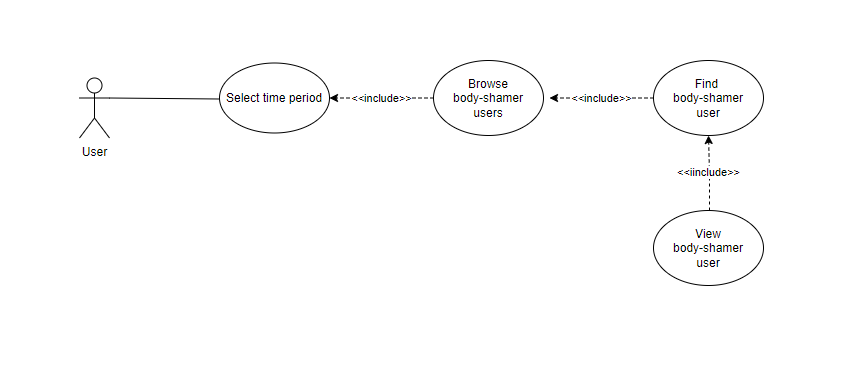
\includegraphics[width= 1.05\textwidth]{images/application/usecases.PNG}
    \caption{Application use cases} 
    \label{application-use-cases}
\end{figure}

\subsection{User Manual}
\begin{figure}[H]
    \centering
    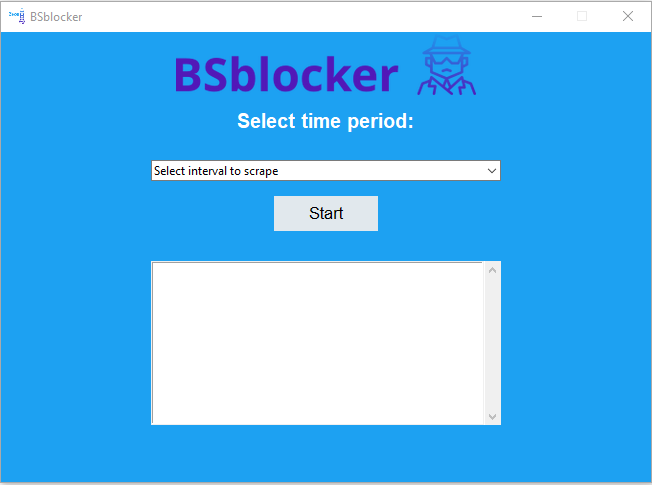
\includegraphics[width= 0.8\textwidth]{images/application/homepage.png}
    \caption{Application home page} 
    \label{application-home}
\end{figure}
\noindent
The user can select a time period in which the application will scan the tweets in order to find out the users that have been done body-shaming. After selecting the period, it is only necessary to press the 'Start' button to let the process start. 
When the detection ends, the name of the users that have done body-shaming appears in the scroll bar below. 

\begin{figure}[H]
    \centering
    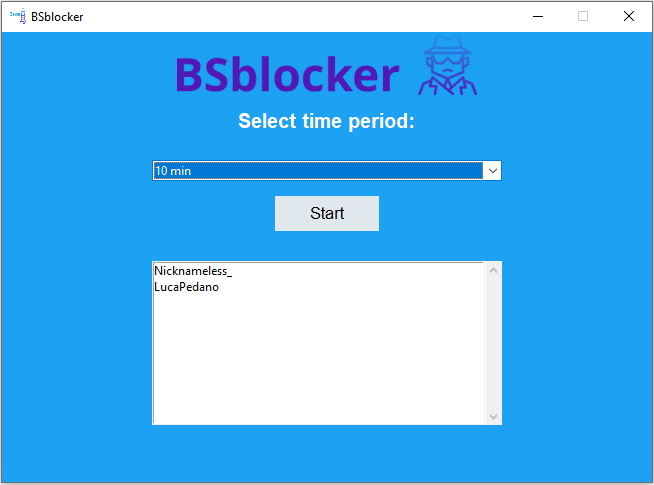
\includegraphics[width= 0.8\textwidth]{images/application/scrape.png}
    \caption{Detection result} 
    \label{use-cases}
\end{figure}

\noindent
When one of the shown users has been detected more than 5 times, it is colored in red.


\begin{figure}[H]
    \centering
    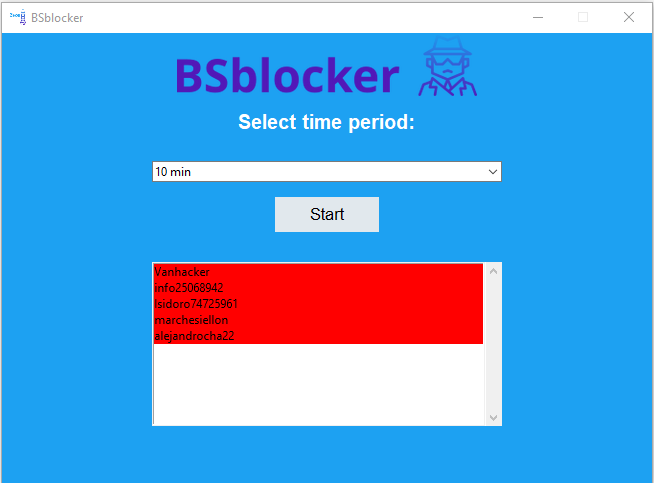
\includegraphics[width= 0.8\textwidth]{images/application/blacklist.PNG}
    \caption{Users in blacklist} 
    \label{application-blacklist}
\end{figure}





